\documentclass[a4paper, 12pt]{article}

\usepackage[utf8]{inputenc}
\usepackage{amsmath}
\usepackage{indentfirst}
\usepackage{graphicx}
\usepackage{multicol,lipsum}
\usepackage{hyperref}
\usepackage{minted}

\begin{document}
%\maketitle

\begin{titlepage}
	\begin{center}
	
	%\begin{figure}[!ht]
	%\centering
	%\includegraphics[width=2cm]{c:/ufba.jpg}
	%\end{figure}

		\Huge{Instituto de Ciências Matemáticas e de Computação}\\
		\large{Departamento de Ciências de Computação}\\ 
		\large{SCC0503 - Algoritmos e Estruturas de Dados II}\\ 
		\vspace{15pt}
        \vspace{95pt}
        \textbf{\LARGE{Relatório Exercício 04}}\\
		%\title{{\large{Título}}}
		\vspace{3,5cm}
	\end{center}
	
	\begin{flushleft}
		\begin{tabbing}
			Alunos: Ryan Souza Sá Teles, Silmar Pereira da Silva Junior \\
            NUSP's: 12822062, 12623950.
			Professor: Leonardo Tórtoro Pereira\\
			%Professor co-orientador: \\
	\end{tabbing}
 \end{flushleft}
	\vspace{1cm}
	
	\begin{center}
		\vspace{\fill}
			 Junho\\
		 2022
			\end{center}
\end{titlepage}
%%%%%%%%%%%%%%%%%%%%%%%%%%%%%%%%%%%%%%%%%%%%%%%%%%%%%%%%%%%

\newpage
% % % % % % % % % % % % % % % % % % % % % % % % % %
\newpage
\tableofcontents
\thispagestyle{empty}

\newpage
\pagenumbering{arabic}
% % % % % % % % % % % % % % % % % % % % % % % % % % %
\section{Introdução}
O exercício consiste na leitura de dados de quests (missões) de um jogo e na construção de um dígrafo capaz de a simular o caminho de execução delas através da travessia em profundidade do dígrafo.\\
Para realizar tal objetivo foi usada a linguagem de programação java, junto ao paradigma de programação orientada a objetos, pois tal combinação permite a estruturação do código de maneira a torna-ló modular e por conseguinte facilitar a manutenção da codebase e compartilhamento da mesma como um pacote ou reusa-lá em mais projetos.\\

\newpage
\section{Desenvolvimento}

O desenvolvimento do projeto fez uso das abstrações já adotadas em sala de aula e o modelo de dígrafo selecionado para trabalhar foi o de "lista de adjâcencias".\\
Tal decisão foi tomada pela comparação entre a complexidade das operações em comparação com a alternativa (matrix de adjacências) e a frequência com que essas operações são feitas.\\
A principail operação realizada durante o algoritimo é a adição de vertices e arestas, em que a lista é O(1) em ambos, já a matriz é $O(|V|^2)$ e O(1) respectivamente. Com relação as demais ambas as abordagens tem complexidades semelhantes.\\
Outro fator que corroborou para a escolha foi a complexidade de espaço entre as opções, com a lista sendo $O(|V|+|E|)$ enquanto a matrix de adjacências sendo $O(|V|^2)$.\\
Com o objetivo de aplicar as boas práticas de código na atividade, foi criado a classe "Answer" que se tornou classe mãe da Vertex, a qual, possui o método "toString" que imprime na tela cada vertice.\\

Implementação da classe Answer:

\begin{minted}[mathescape, linenos]{java}

public class Answer {
    private int id;
    private String name;
    private String description;
    
    public Answer(int id, String name, String description) {
        this.id = id;
        this.name = name;
        this.description = description;
    }
    
    public int getId() {return id;}
    public String getName() {return name;}
    public String getDescription() {return description;}
    public void setId(int id) {this.id = id;}
    public void setName(String name) {this.name = name;}
    
    public void setDescription(String description) {
        this.description = description;
    }
    public String toString() {
        return "Quest{\n\tID: " + id + "\n\tName: " + name + "\n\tDescription: " + description + "\n}";
    }
}


\end{minted}


Para a implementação do algoritmo de busca em profundidade, por questões didáticas e não de desempenho algorítmico, foi criado o método "getAllConnectedVertex" dentro da classe "DigraphList" e definido seu contrato na interface "GraphInterface", abaixo a implementação:

\begin{minted}[mathescape, linenos]{java}
    public List<Vertex> getAllConnectedVertex(Vertex vertex) {
        if (getAdjacencyList().get(getVertices().indexOf(vertex)).isEmpty()) {
            return Collections.emptyList();
        } else {
            List<Vertex> connectedVertices = new ArrayList<>();
            int vertexIndex = getVertices().indexOf(vertex);
            for (Edge edge : getAdjacencyList().get(vertexIndex)) {
                connectedVertices.add(edge.getDestination());
            }
            return connectedVertices;
        }
    }
\end{minted}

A implementação do algoritmo Depth First Search: 

\begin{minted}[mathescape, linenos]{java}
public void traverseGraph(Vertex source) {
        depthFirstTraversalRecursive(source);
        printPath();
    }

    public void depthFirstTraversalRecursive(Vertex source) {
        int sourceIndex = getGraph().getVertices().indexOf(source);
        addToPath(source);
        markVertexAsVisited(sourceIndex);
        setDistanceToVertex(sourceIndex, 0);
        setPredecessorVertexIndex(sourceIndex, -1);

        List<Vertex> vertexesToVisit = getGraph().getAllConnectedVertex(source);

        for (Vertex currentVisitedVertex : vertexesToVisit) {
            if (!hasVertexBeenVisited(getGraph().getVertices().indexOf(currentVisitedVertex))) {
                depthFirstTraversalRecursive(currentVisitedVertex);
            }
        }
    }
\end{minted}

Como modelo de busca recursiva para o algoritmo, ele sempre vai estar indo do primeiro vertice adicionado como aresta a partir do vértice de origem.

\newpage
\section{Resultados}
\graphicspath{ {./Results/} }

Para o caso de teste 1 temos como saída:
\begin{minted}{xml}
    INFO: Quest{
	ID: 8
	Name: Elder Care
	Description: Help the village Elder
}Quest{
	ID: 9
	Name: Second Intentions
	Description: Make the Elder tell you about the Demon Lord
}Quest{
	ID: 5
	Name: Hell's Door
	Description: You must find the entrance to the Demon Lord's Castle
}Quest{
	ID: 6
	Name: Cleaning the House
	Description: Kill all the guardians of the Demon Lord
}Quest{
	ID: 7
	Name: Showdown
	Description: Face the last fierce battle and kill the Demon Lord
}
\end{minted}

Quanto ao grafo gerado:

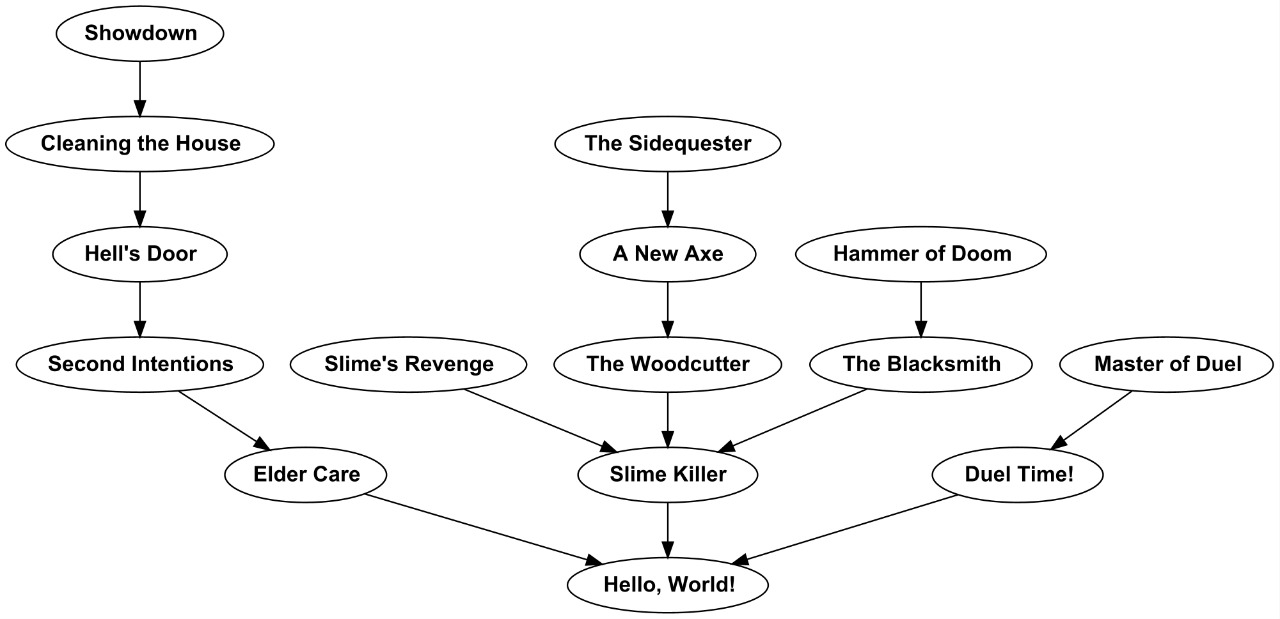
\includegraphics[width=\textwidth]{Case1.jpeg}
\\
\\

\newpage
Para o caso 2 temos como saída:

\begin{minted}{xml}
    INFO: Quest{
	ID: 0
	Name: Slime Killer
	Description: You must kill 10 slimes
}Quest{
	ID: 11
	Name: Slime's Revenge
	Description: The slime Queen wants revenge for her minions
}Quest{
	ID: 1
	Name: The Woodcutter
	Description: Find and talk to Greyson, the woodcutter
}Quest{
	ID: 2
	Name: A New Axe
	Description: Search for the legendary axe for Greyson
}Quest{
	ID: 3
	Name: The Blacksmith
	Description: Find and talk to Clint, the blacksmith
}Quest{
	ID: 4
	Name: Hammer of Doom
	Description: Search for the legendary hammer for Clint
}
\end{minted}

Quanto a seu grafo:\\

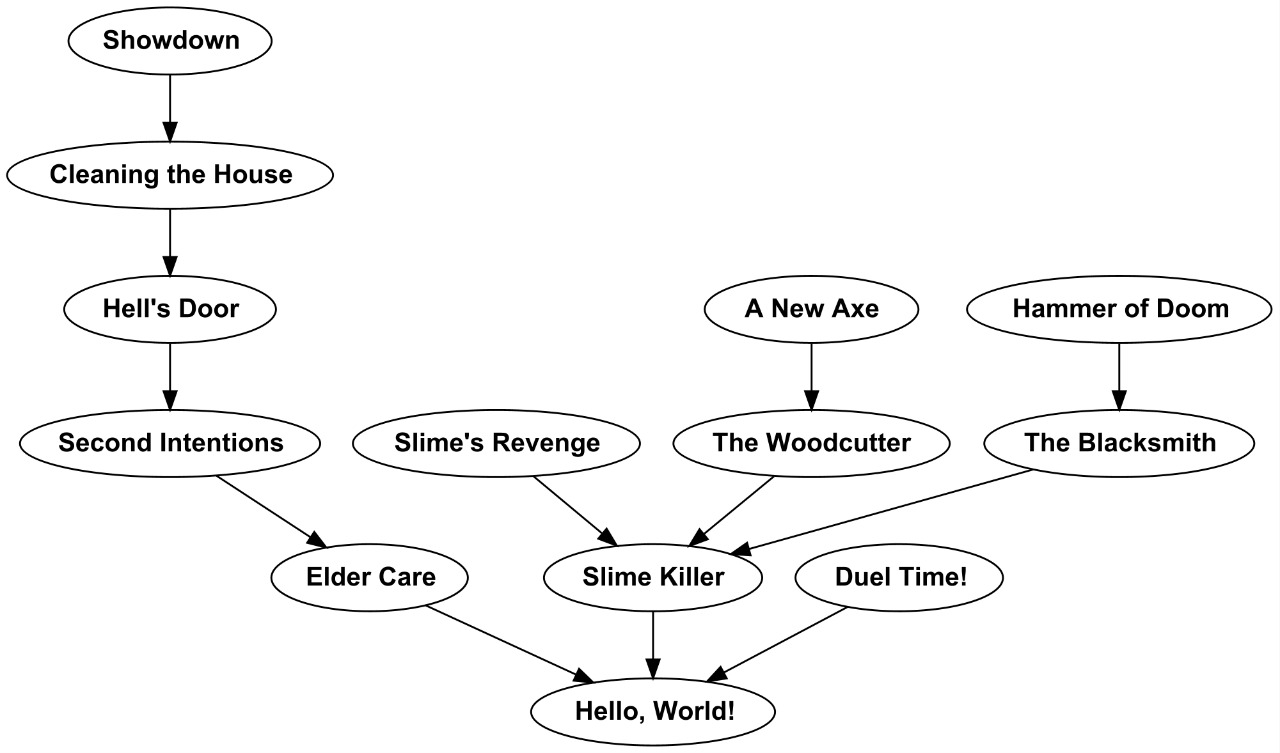
\includegraphics[width=\textwidth]{Case2.jpeg}
\\
\\

\newpage
Para o caso 3 temos como saída:


\begin{minted}{xml}
    INFO: Quest{
	ID: 10
	Name: Hello, World!
	Description: Get to the starter town and talk to the villagers
}Quest{
	ID: 0
	Name: Slime Killer
	Description: You must kill 10 slimes
}Quest{
	ID: 11
	Name: Slime's Revenge
	Description: The slime Queen wants revenge for her minions
}Quest{
	ID: 1
	Name: The Woodcutter
	Description: Find and talk to Greyson, the woodcutter
}Quest{
	ID: 2
	Name: A New Axe
	Description: Search for the legendary axe for Greyson
}Quest{
	ID: 14
	Name: The Sidequester
	Description: Face the final challenge and complete the last sidequest
}Quest{
	ID: 3
	Name: The Blacksmith
	Description: Find and talk to Clint, the blacksmith
}Quest{
	ID: 4
	Name: Hammer of Doom
	Description: Search for the legendary hammer for Clint
}Quest{
	ID: 12
	Name: Duel Time!
	Description: Win the card minigame tournament
}Quest{
	ID: 13
	Name: Master of Duel
	Description: Win the world championship card minigame tournament
}Quest{
	ID: 8
	Name: Elder Care
	Description: Help the village Elder
}Quest{
	ID: 9
	Name: Second Intentions
	Description: Make the Elder tell you about the Demon Lord
}Quest{
	ID: 5
	Name: Hell's Door
	Description: You must find the entrance to the Demon Lord's Castle
}Quest{
	ID: 6
	Name: Cleaning the House
	Description: Kill all the guardians of the Demon Lord
}Quest{
	ID: 7
	Name: Showdown
	Description: Face the last fierce battle and kill the Demon Lord
}
\end{minted}


Para seu grafo Temos:\\
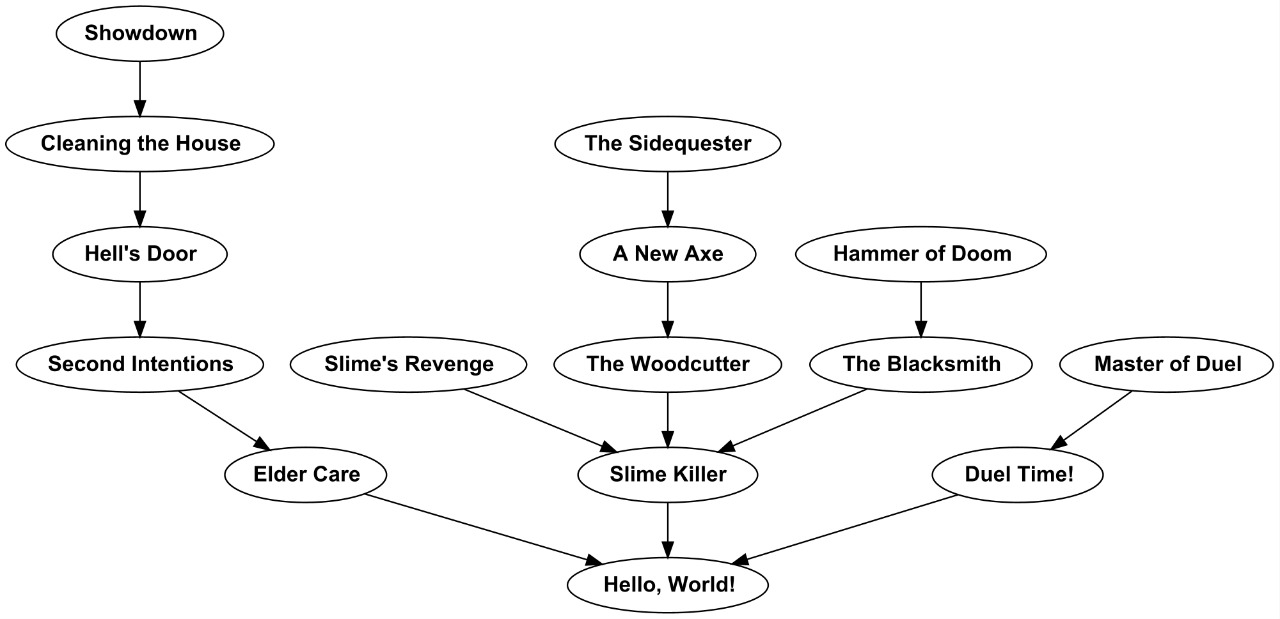
\includegraphics[width=\textwidth]{Case3.jpeg}
\\
\\


\newpage
Por fim para o caso 4 temos como saida:
\begin{minted}{xml}
    INFO: Quest{
	ID: 10
	Name: Hello, World!
	Description: Get to the starter town and talk to the villagers
}Quest{
	ID: 0
	Name: Slime Killer
	Description: You must kill 10 slimes
}Quest{
	ID: 11
	Name: Slime's Revenge
	Description: The slime Queen wants revenge for her minions
}Quest{
	ID: 1
	Name: The Woodcutter
	Description: Find and talk to Greyson, the woodcutter
}Quest{
	ID: 2
	Name: A New Axe
	Description: Search for the legendary axe for Greyson
}Quest{
	ID: 3
	Name: The Blacksmith
	Description: Find and talk to Clint, the blacksmith
}Quest{
	ID: 4
	Name: Hammer of Doom
	Description: Search for the legendary hammer for Clint
}Quest{
	ID: 12
	Name: Duel Time!
	Description: Win the card minigame tournament
}Quest{
	ID: 8
	Name: Elder Care
	Description: Help the village Elder
}Quest{
	ID: 9
	Name: Second Intentions
	Description: Make the Elder tell you about the Demon Lord
}Quest{
	ID: 5
	Name: Hell's Door
	Description: You must find the entrance to the Demon Lord's Castle
}Quest{
	ID: 6
	Name: Cleaning the House
	Description: Kill all the guardians of the Demon Lord
}Quest{
	ID: 7
	Name: Showdown
	Description: Face the last fierce battle and kill the Demon Lord
}
\end{minted}

Para seu grafo Temos:\\
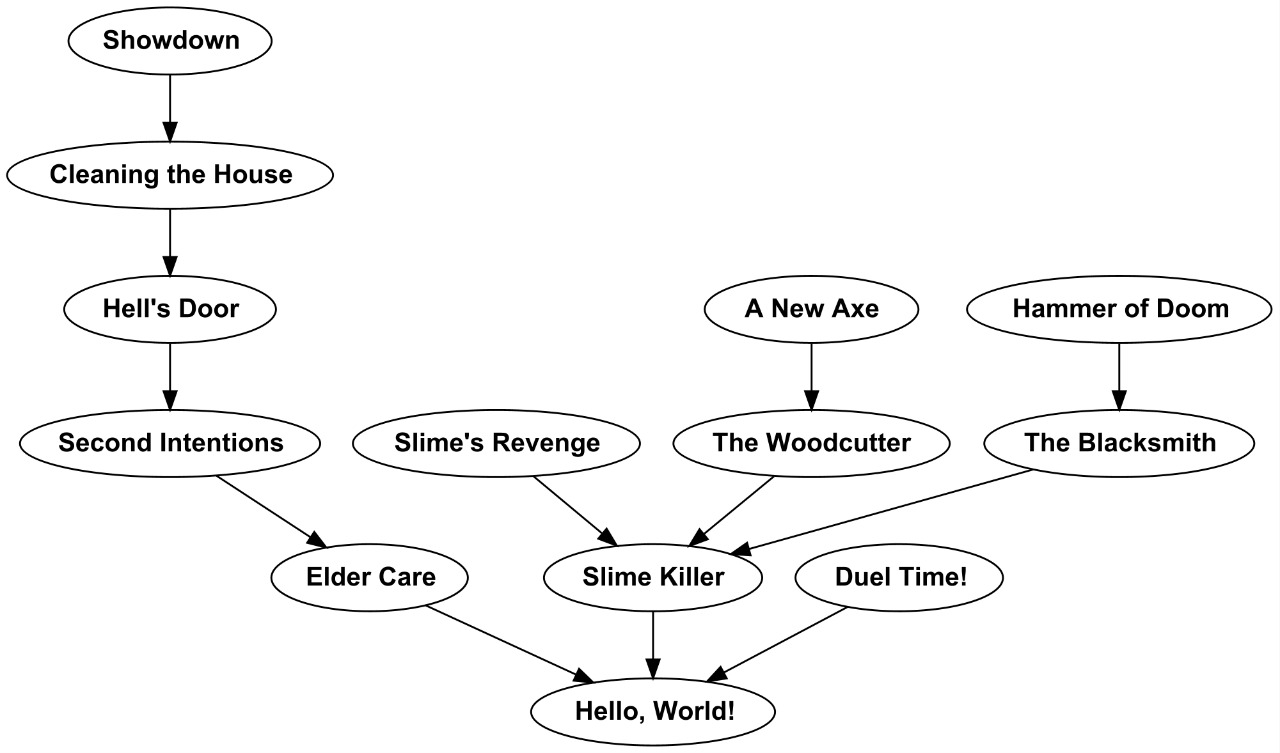
\includegraphics[width=\textwidth]{Case4.jpeg}
\\
\\
\end{document}



